\documentclass[aspectratio=169,10pt]{beamer}

\usepackage[utf8]{inputenc}
\usepackage[T1]{fontenc}
\usepackage[spanish,es-nodecimaldot]{babel}
\usepackage{amsmath}
\usepackage{booktabs}
\usepackage{tikz}
\usepackage{graphicx}
\usetikzlibrary{arrows.meta}
\useoutertheme[subsection=false,footline=empty]{miniframes}

% Estilo Beamer sencillo, inspirado en las diapositivas interiores de K_SVC.pdf.
\setbeamertemplate{navigation symbols}{}
\setbeamertemplate{frametitle}{%
  \vspace{.28cm}\begin{center}\normalfont\Large\insertframetitle\end{center}\vspace{.15cm}}
\setbeamercolor{normal text}{fg=black,bg=white}
\setbeamercolor{frametitle}{fg=black,bg=white}
\setbeamercolor{itemize item}{fg=black}
\setbeamercolor{section in head/foot}{fg=black,bg=white}
\setbeamercolor{mini frame}{fg=black,bg=white}
\setbeamercolor{upper separation line head}{bg=white}
\setbeamercolor{middle separation line head}{bg=white}
\setbeamercolor{lower separation line head}{bg=white}
\setbeamertemplate{itemize item}{\raise0.15ex\hbox{\large$\bullet$}}
\setbeamertemplate{footline}{}
\setbeamersize{text margin left=1.0cm,text margin right=1.0cm}
\renewcommand{\familydefault}{\sfdefault}

\newcommand{\metric}[2]{\textbf{#1}\quad #2}

\begin{document}

% 1. Resumen del trabajo y resultados
\section{Resumen}
\begin{frame}
  \vspace{.35cm}
  \begin{center}
    {\LARGE Predicción de la dificultad de pago}\\[.22cm]
    {\normalsize Inteligencia Artificial Explicable --- Unidad 2, Fase II}\\[.35cm]
    {\small Damián Benasco Sánchez \quad Germán Sánchez Carmona \quad Jorge Enrique Vega Ortiz}\\[.6cm]

    {\large Resultados de validación cruzada externa}\\[.15cm]
    \renewcommand{\arraystretch}{1.45}
    \begin{tabular}{@{}lr@{}}
      \toprule
      Modelo & ROC-AUC medio \\
      \midrule
      CART & 0,7372 \\
      Regresión logística & 0,7515 \\
      \textbf{EBM} & \textbf{0,7755} \\
      \bottomrule
    \end{tabular}\\[.42cm]
    \textbf{Modelo elegido: EBM, por su mejor rendimiento y capacidad de interpretación.}
  \end{center}
\end{frame}

% 2. Árbol CART
\section{CART}
\begin{frame}{Árbol de decisión (CART)}
  \begin{center}
    Cada hoja muestra la probabilidad estimada $P(1)$.\\[.05cm]
    \begin{tikzpicture}[
      split/.style={align=center,text width=2.1cm,font=\small,inner sep=2pt},
      root/.style={split,text width=2.35cm},
      leaf/.style={align=center,text width=1.0cm,font=\small,inner sep=3pt},
      edge/.style={-{Stealth[length=1.7mm]},draw=black,line width=.55pt},
      branch/.style={font=\footnotesize,fill=white,inner sep=1pt}
    ]
      \node[root] (r) at (6.1,0) {Estado reciente\\$\leq 0{,}5$?};
      \node[split] (r0) at (3.0,-1.12) {Pago/factura (6m)\\$\leq 0{,}105$?};
      \node[split] (r1) at (9.2,-1.12) {Pago/factura (6m)\\$\leq 0{,}105$?};
      \node[split] (a) at (1.45,-2.28) {Meses sin pago\\$\leq 3{,}5$?};
      \node[split] (b) at (4.55,-2.28) {Meses sin pago\\$\leq 2{,}5$?};
      \node[split] (c) at (7.65,-2.28) {Meses sin pago\\$\leq 2{,}5$?};
      \node[split] (d) at (10.75,-2.28) {Meses sin pago\\$\leq 2{,}5$?};
      \draw[edge] (r) -- node[branch,above left]{sí} (r0);
      \draw[edge] (r) -- node[branch,above right]{no} (r1);
      \draw[edge] (r0) -- node[branch,above left]{sí} (a);
      \draw[edge] (r0) -- node[branch,above right]{no} (b);
      \draw[edge] (r1) -- node[branch,above left]{sí} (c);
      \draw[edge] (r1) -- node[branch,above right]{no} (d);
      \node[leaf] (l1) at (.7,-3.48) {0,192};
      \node[leaf] (l2) at (2.2,-3.48) {0,406};
      \node[leaf] (l3) at (3.8,-3.48) {0,072};
      \node[leaf] (l4) at (5.3,-3.48) {0,121};
      \node[leaf] (l5) at (6.9,-3.48) {0,465};
      \node[leaf] (l6) at (8.4,-3.48) {0,693};
      \node[leaf] (l7) at (10.0,-3.48) {0,193};
      \node[leaf] (l8) at (11.5,-3.48) {0,283};
      \draw[edge] (a) -- node[branch,above left]{sí} (l1.north);
      \draw[edge] (a) -- node[branch,above right]{no} (l2.north);
      \draw[edge] (b) -- node[branch,above left]{sí} (l3.north);
      \draw[edge] (b) -- node[branch,above right]{no} (l4.north);
      \draw[edge] (c) -- node[branch,above left]{sí} (l5.north);
      \draw[edge] (c) -- node[branch,above right]{no} (l6.north);
      \draw[edge] (d) -- node[branch,above left]{sí} (l7.north);
      \draw[edge] (d) -- node[branch,above right]{no} (l8.north);
    \end{tikzpicture}
  \end{center}
  \vspace{-.08cm}
  \begin{center}
    \metric{ROC-AUC}{0,7372 $\pm$ 0,0044}\qquad
    \metric{Balanced accuracy}{67,3\%}\qquad
    \metric{Sensibilidad}{48,9\%}\\[.08cm]
    {\footnotesize Validación externa en cinco particiones; métricas de clasificación con umbral 0,25.}
  \end{center}
\end{frame}

% 3. Regresión logística
\section{Regresión logística}
\begin{frame}{Regresión logística}
  \vspace{-.25cm}
  \begin{center}
    {\large $\displaystyle \log\!\left(\frac{p}{1-p}\right)=\beta_0+\sum_j\beta_j z_j$}\\[.18cm]
    Un coeficiente positivo aumenta la puntuación en log-odds; uno negativo la reduce.
  \end{center}
  \vspace{.4cm}
  \begin{columns}[T,onlytextwidth]
    \begin{column}{.61\textwidth}
      {\large\bfseries Variables más relevantes}
      \begin{itemize}\setlength\itemsep{.45em}
        \item Más meses sin pago, un estado de pago reciente más alto y mayor utilización se asocian con una puntuación mayor.
        \item El plan de asistencia también tiene coeficiente positivo.
        \item Un total pagado mayor se asocia con una puntuación menor, manteniendo las demás variables constantes.
      \end{itemize}
    \end{column}
    \begin{column}{.35\textwidth}
      {\large\bfseries Resultados}\\[.2cm]
      \metric{ROC-AUC}{0,7515 $\pm$ 0,0075}\\[.28cm]
      \metric{Balanced accuracy}{68,1\%}\\[.22cm]
      \metric{Sensibilidad}{59,6\%}\\[.3cm]
      {\footnotesize Media externa de cinco particiones. Umbral seleccionado en cada entrenamiento.}
    \end{column}
  \end{columns}
\end{frame}

% 4. EBM
\section{EBM}
\begin{frame}{Explainable Boosting Machine (EBM)}
  \begin{center}\small
    EBM aprende una función para cada variable y suma sus aportes en log-odds:\\[-.02cm]
    $\operatorname{logit}(p)=\beta_0+\sum_{j=1}^{15} f_j(x_j)$\quad (\texttt{interactions=0})
  \end{center}
  \vspace{-.4cm}
  \begin{center}
    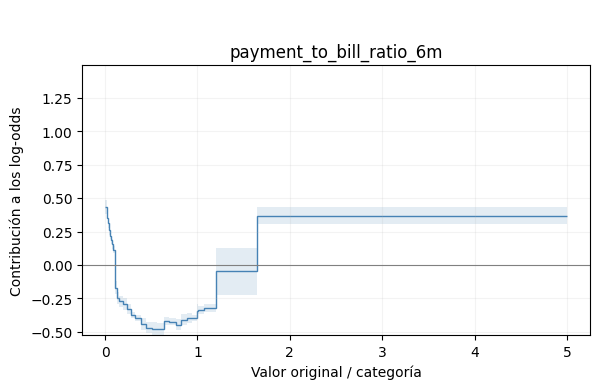
\includegraphics[height=4.2cm,width=.88\textwidth,keepaspectratio]{ebm_payment_to_bill_ratio.png}\\[-.12cm]
    {\scriptsize El aporte del cociente pagos/facturas varía con su valor (partición 1).}
  \end{center}
  \vspace{-.22cm}
  \begin{center}
    \metric{ROC-AUC}{0,7755 $\pm$ 0,0077}\qquad
    \metric{Balanced accuracy}{70,0\%}\qquad
    \metric{F1}{0,507}\\[.02cm]
    {\scriptsize Media externa de cinco particiones. EBM fue el modelo elegido.}
  \end{center}
\end{frame}

\end{document}
